\documentclass[spanish]{beamer}
\usepackage[utf8]{inputenc}
\usepackage[spanish]{babel}
\usepackage{upgreek}
\usepackage{mathtools}
\usepackage{svg}   

\usetheme{Madrid}
\usecolortheme{beaver}



\title{Introducción a la Teoría de Código}
\author{Angel Granados \\ Nicolas Siatama \\ Valentina Vivas}
\institute{Universidad Distrital Francisco José de Caldas \\ Gabriel Bravo Ríos}
\date{\today}

\begin{document}
	
	\frame{\titlepage}
	
	\begin{frame}
	\frametitle{Códigos de Corrección de Errores}
	
	Los Códigos de Corrección de Errores se utiliza para corregir errores cuando los mensajes se transmiten a través de un canal \textbf{Ruidoso}. \vspace{0.5cm}
	
	Un canal puede ser:
	
	
	
{
	\centering
	
	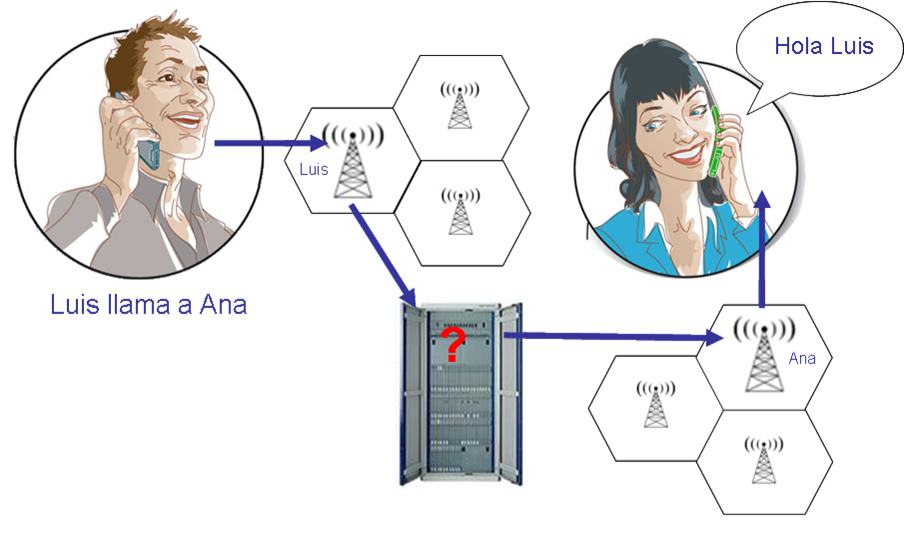
\includegraphics[width=0.5\linewidth]{img/img1}

}	
\end{frame}

\begin{frame}
	\frametitle{Ejemplo de Transmisión de mensajes}
	
	
	{	
		
		\centering
		
		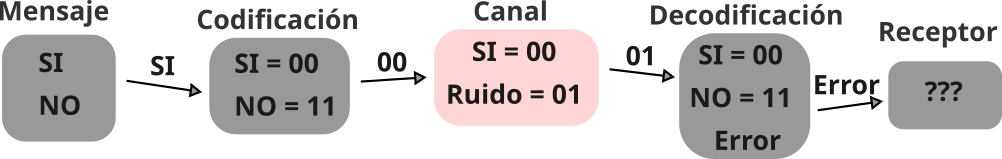
\includegraphics[width=0.7\linewidth]{img/img2}
		
		
	}


{

\huge

\centering

\vspace*{0.5cm} 
¿Cómo se soluciona?
	
}	
\end{frame}


\begin{frame}
	\frametitle{Ejemplo de Transmisión de mensajes}
	
		{
		
		\huge
		
		\centering
		
		Agregando más 0s y 1s
		\vspace*{0.5cm} 
		
	}
	
	
	
	{	
		
		\centering
		
		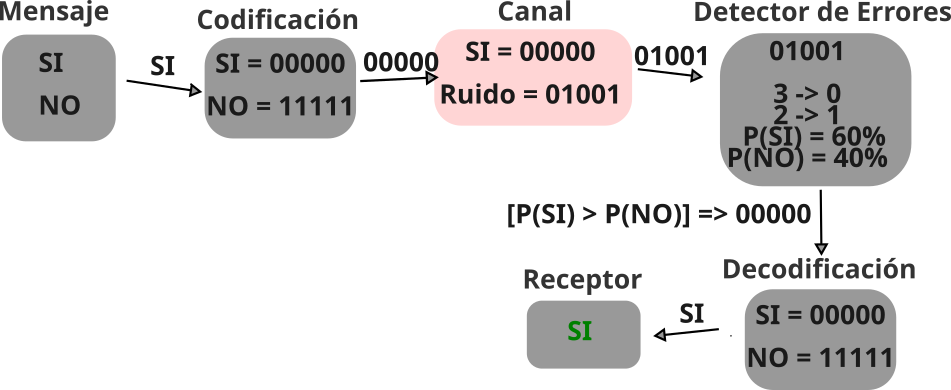
\includegraphics[width=0.7\linewidth]{img/img21}
		
		
	}
	
	
	
\end{frame}


\begin{frame}
	\frametitle{Ejemplo de un Canal sin Códigos de Corrección de Errores}
	
	
{	

	\centering
	
	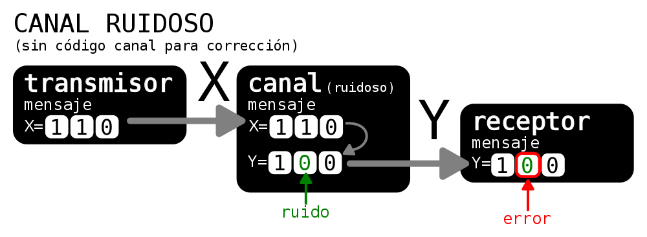
\includegraphics[width=0.7\linewidth]{img/img3}


}

	
\end{frame}

\begin{frame}
	\frametitle{Redundancia}
	
	
	De los ejemplos anteriores, el \textbf{código} se denomina \textbf{código de repetición} y tenemos códigos longitudes de 2,5 y 3.
	
	\vspace*{0.5cm}
	
	La importancia de añadir \textbf{redundancia} a los mensajes es protegerlos contra el ruido.
	
	
\end{frame}
	\include{nicolas}
	\include{valentina}
	 
	
	\begin{frame}
		\frametitle{Introducción}
		Este es un texto en la primera diapositiva.
	\end{frame}
	
\end{document}
